\part{The x86 CPU Architecture}
\frame{\partpage}

\begin{frame}{Intel x86}
    \begin{itemize}
        \pause\item Introduced in 1978 with the Intel 8086 (16-bit)
        \pause\item Extended to 32-bit in 1985 with the Intel 80306
        \pause\item Extended to 64-bit (x86-64 or x64) in 2003 with the AMD Opteron
    \end{itemize}
\end{frame}

\begin{frame}{Uses of Intel x86}
	\begin{columns}
		\begin{column}{0.32\textwidth}
			\pause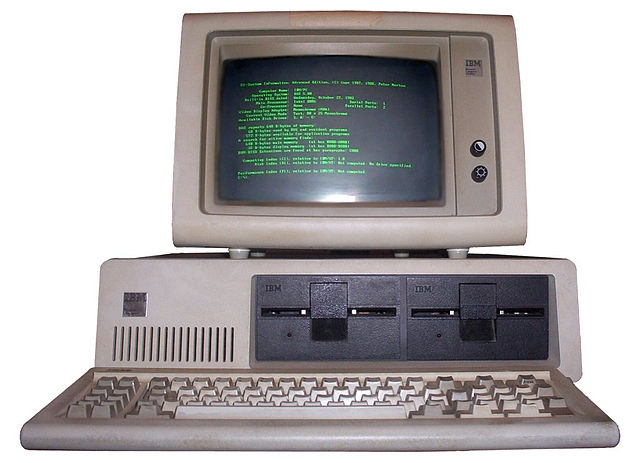
\includegraphics[width=\textwidth]{ibm_5150}
		\end{column}
		\begin{column}{0.32\textwidth}
			\pause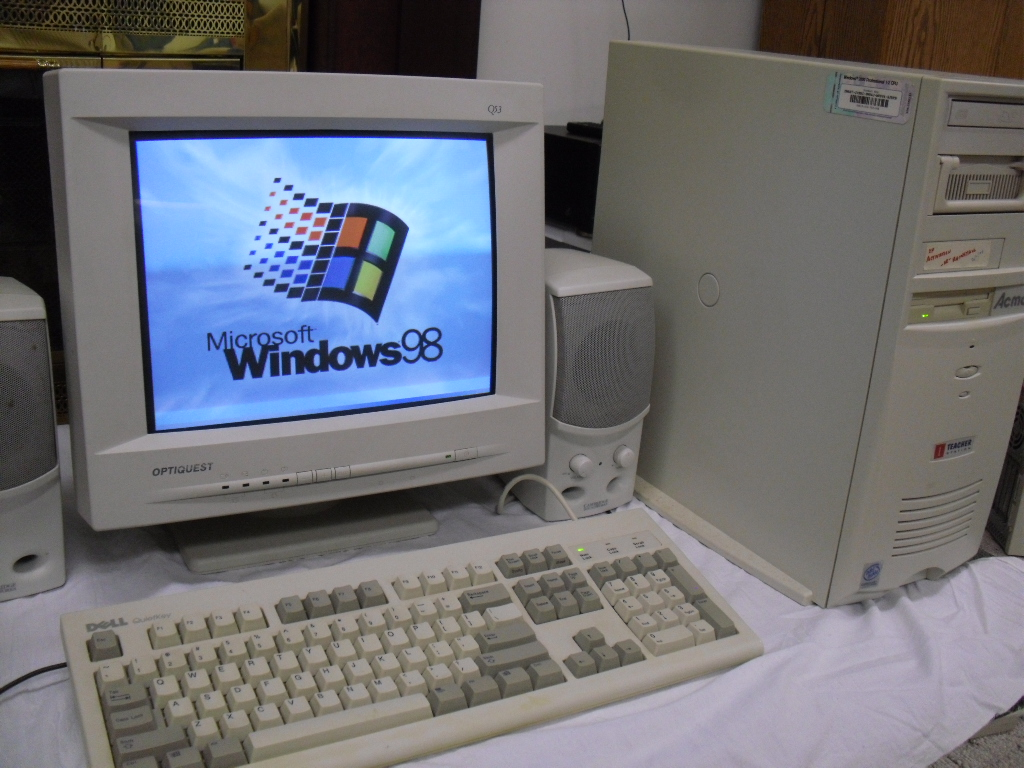
\includegraphics[width=\textwidth]{windows_98}
		\end{column}
		\begin{column}{0.32\textwidth}
			\pause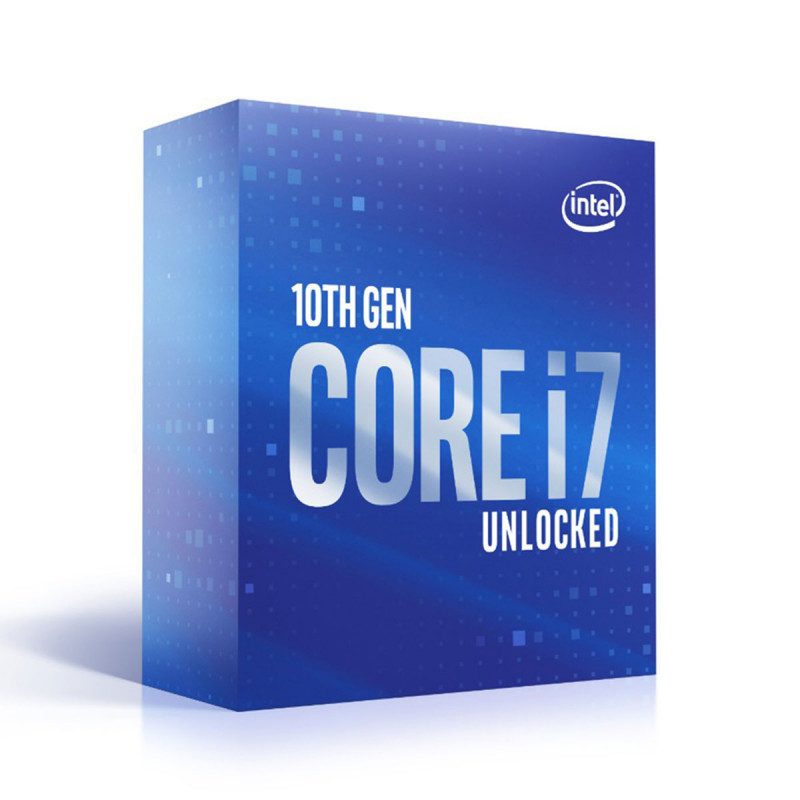
\includegraphics[width=\textwidth]{intel_i7}
		\end{column}
	\end{columns}
	\begin{columns}
		\begin{column}{0.32\textwidth}
			\pause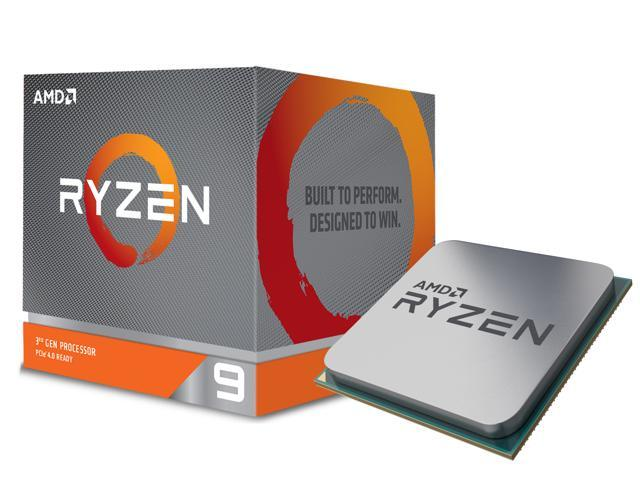
\includegraphics[width=\textwidth]{amd_ryzen}
		\end{column}
		\begin{column}{0.32\textwidth}
			\pause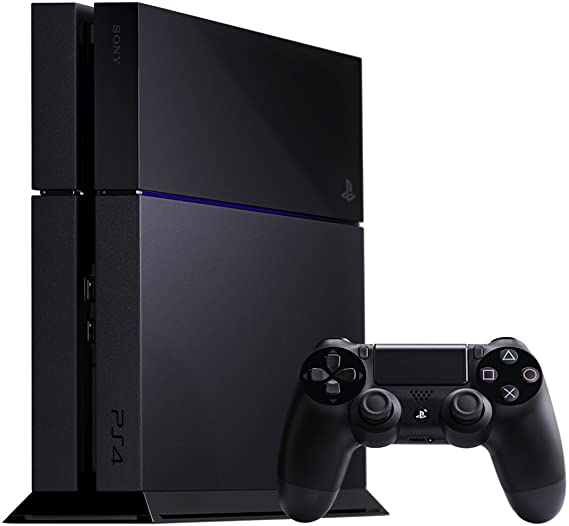
\includegraphics[width=\textwidth]{ps4}
		\end{column}
		\begin{column}{0.32\textwidth}
			\pause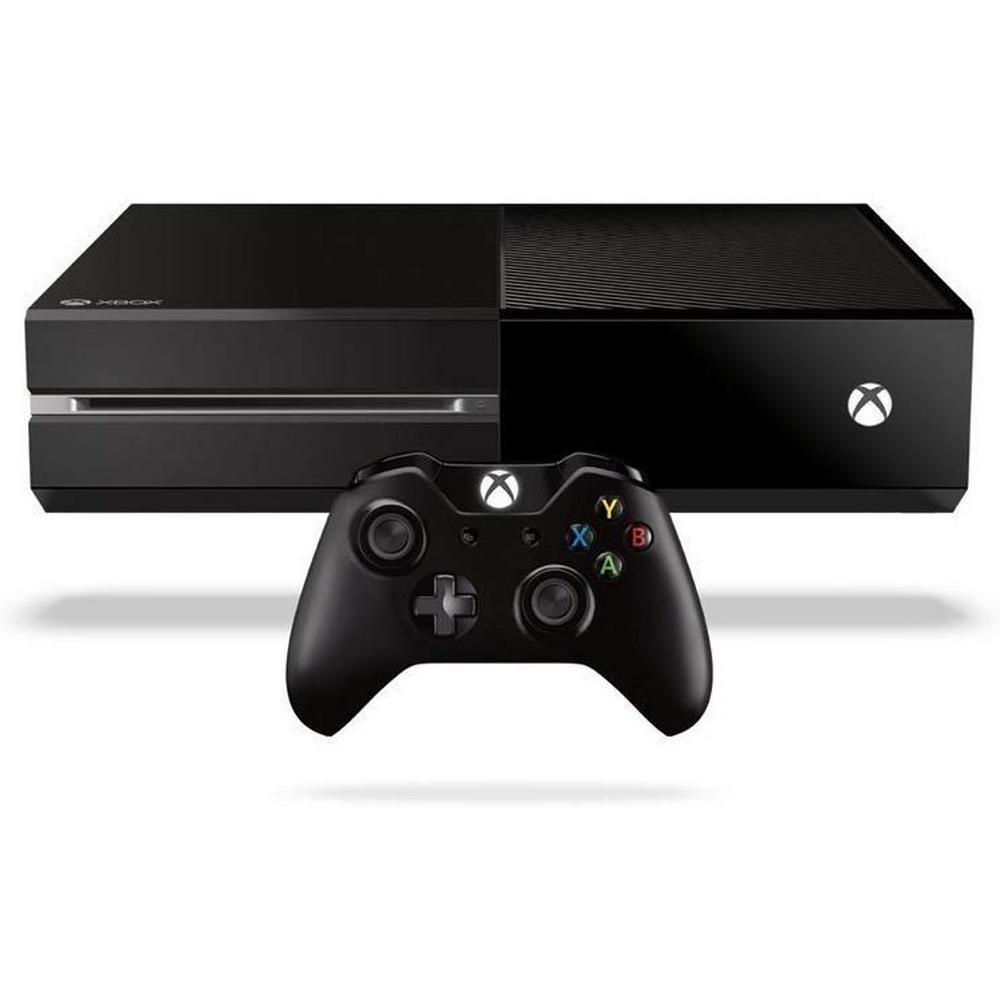
\includegraphics[width=\textwidth]{xbox_one}
		\end{column}
	\end{columns}
\end{frame}

\begin{frame}{Backwards compatibility}
    \begin{itemize}
        \pause\item New CPUs have built upon the x86 instruction set over the years
        \pause\item x86-64 includes 64, 32 and 16-bit instructions
        \pause\item Technically, a PC from \the\year{} could run the same OS and software as the IBM 5150
    \end{itemize}
\end{frame}

\begin{frame}{Features of modern x86-64}
    \begin{itemize}
        \pause\item x87 floating point unit
            \begin{itemize}
                \pause\item Hardware support for IEEE754 floating point
            \end{itemize}
        \pause\item SIMD instructions
            \begin{itemize}
                \pause\item SIMD = Single Instruction, Multiple Data
                \pause\item E.g.\ one instruction to multiply 4 pairs of numbers in parallel
            \end{itemize}
        \pause\item Security features
            \begin{itemize}
                \pause\item AES encryption and decryption
                \pause\item Secure random number generation
            \end{itemize}
        \pause\item Multiple cores and hyperthreading
            \begin{itemize}
                \pause\item CPU can do more than one thing at once
            \end{itemize}
    \end{itemize}
\end{frame}
